\documentclass[runningheads]{llncs}
\usepackage[utf8]{inputenc}
\usepackage[T1]{fontenc}
\usepackage[a4paper,margin=2.5cm]{geometry}
\usepackage{amsmath}
\usepackage{amssymb}
\usepackage{enumitem}
\usepackage{booktabs}
\usepackage{array}
\usepackage{url}
\usepackage{graphicx}
\usepackage{algorithm}
\usepackage{algpseudocode}
\usepackage{tikz}
\usetikzlibrary{positioning,arrows.meta,fit}
\usepackage[hidelinks]{hyperref}

\setlist{itemsep=2pt, topsep=4pt}

\begin{document}

\title{Lymphoma Subtype Classification from Multi-Platform DNA Methylation Data: Data Harmonization and Leakage-Free Evaluation}
\titlerunning{Lymphoma Classification from Methylation Data}

\author{Diana Timiș}
\authorrunning{D. Timiș}

\institute{Department of Computer Science, Faculty of Mathematics and Computer Science,\\
Babeș-Bolyai University, Cluj-Napoca, Romania\\
\email{diana.timis1@stud.ubbcluj.ro}}

\maketitle

\section{Related Work}\label{sec:related}

\subsection{Machine Learning on DNA Methylation Data}
A systematic review~\cite{yuan2023} of 83 epigenome-wide studies identifies three main workflows: unsupervised clustering, supervised feature selection and deep feature transformation. It also reports that the performance of the models is often not evaluated adequately. Celli et al.~\cite{celli2018} classify breast, kidney and thyroid carcinomas from array data with decision trees and random forests, and extract several equally accurate models by iteratively removing the selected features. De Velasco et al.~\cite{develasco2024} reduce the CpG sites of 890 TCGA array samples (10 cancer types) to 100 with ANOVA, gain ratio and a gradient boosting selector, and classify them with XGBoost, CatBoost and random forest. Newsham et al.~\cite{newsham2024} select informative loci with XGBoost and classify 13 cancer types and normal tissue with a deep neural network.

\subsection{Methylation-Based Studies of Lymphoma}
Espín-Pérez et al.~\cite{espinperez2022} predict the future development of B-cell non-Hodgkin lymphoma from peripheral blood arrays with a score based on 135 CpG sites. Glaser et al.~\cite{glaser2025} derive methylation modules with machine learning to subgroup germinal-centre-derived B-cell lymphomas (follicular lymphoma, DLBCL and transformed cases) from 450K array data, and Queirós et al.~\cite{queiros2016} identify subgroups of mantle cell lymphoma. An existing baseline pipeline, which is not yet published, aggregates sequencing data into differentially methylated regions (DMRs), selects features with variance filtering and mRMR and classifies the samples with XGBoost on a single train/test split.

\subsection{Comparison with the Proposed Approach}
Table~\ref{tab:related} compares these approaches with the one proposed here. The similarities are the use of feature selection before classification and of tree ensembles (XGBoost, random forest). The differences are the data and the evaluation: the existing studies use large cohorts measured on one platform, report mainly the accuracy and do not target lymphoma subtyping from several platforms.

\begin{table}[!htb]
\centering
\caption{Approaches compared with this work.}
\label{tab:related}
\small
\begin{tabular}{>{\raggedright\arraybackslash}p{2.2cm}>{\raggedright\arraybackslash}p{3.0cm}>{\raggedright\arraybackslash}p{3.5cm}>{\raggedright\arraybackslash}p{2.5cm}>{\raggedright\arraybackslash}p{2.6cm}}
\toprule
Work & Data & Features and model & Validation & Reported result \\
\midrule
Celli et al.~\cite{celli2018} & TCGA arrays, 3 carcinomas & Iterative decision trees, random forest & Single-platform cohorts & Accuracy above 97\% \\
De Velasco et al.~\cite{develasco2024} & 890 TCGA arrays, 10 cancer types & ANOVA, gain ratio, 100 CpGs; XGBoost, CatBoost, RF & 5-fold CV and test set & Accuracy 87.7--93.5\% \\
Newsham et al.~\cite{newsham2024} & Arrays, 13 cancer types and normal & XGBoost selection, deep neural network & 25\% test set, external datasets & Accuracy 98.2\% \\
Espín-Pérez et al.~\cite{espinperez2022} & Blood arrays, 278 individuals & 135-CpG score & Validation cohort & Accuracy 78--85\% (future), 96.3\% (active lymphoma) \\
Glaser et al.~\cite{glaser2025} & 450K arrays, 177 lymphomas & Machine-learning methylation modules & Cohort analysis & Subgroups of FL and DLBCL \\
Baseline (unpublished) & Sequencing, 30 samples (later 315) & DMRs, variance + mRMR, XGBoost & Single 252/63 split & Not yet published \\
This work & Arrays, RRBS, WGBS; several genome builds & DMRs or annotated regions, mRMR, XGBoost & Nested CV, leakage-free; leaky variant & Macro F1, MCC, stability (Section~\ref{sec:case}) \\
\bottomrule
\end{tabular}
\end{table}

\subsection{Where Similar or Better Results Are Expected}
\begin{itemize}
\item \textbf{Accuracy and macro F1.} Results \emph{lower than or similar to} those of the array studies are expected: their cohorts contain hundreds of samples from one platform, while ours contains few samples from several platforms, and our estimates are not inflated by leakage.
\item \textbf{Reliability of the estimates.} \emph{Better} results are expected: nested cross-validation reports a mean and a standard deviation over folds instead of a single test score, and all data-dependent steps are fitted on the training samples only.
\item \textbf{Robustness across platforms.} This aspect is not measured by the other studies; it is measured here by the overlap of the regions (E2), by the grouping of the samples (E3) and, on larger data, by leave-one-dataset-out evaluation (E6).
\item \textbf{Stability of the selected features.} It is rarely reported; it is measured here with the Jaccard index across folds~\cite{nogueira2018}.
\end{itemize}

\subsection{Preparation of the Validation on Larger Data}\label{sec:validation}

The case study uses a small public dataset; the experimental validation will repeat the experiments on larger data. The dataset of the baseline (315 samples, eight classes) is not public, so the validation will use larger public datasets and, if available, a subset of the baseline data. The pipeline is ready for this: the datasets are described in a configuration file, array matrices with one column per sample are supported, and an experiment configuration with E0 and the thresholds for arrays is part of the repository. The planned steps are: (i)~converting the new datasets and checking them with E1, in particular the 450K data of GSE276853 (follicular lymphoma and DLBCL) and the EM-seq normal samples of GSE259312; (ii)~running E2--E5 on the extended data, with the small classes merged into \emph{other lymphoma}; (iii)~running E6 for the classes measured in several datasets, e.g.\ DLBCL and normal samples, which breaks the confounding between class and dataset of the case study; and (iv)~reproducing the baseline (E0) if its data and its train/test split become available. GSE276853 is the dataset of Glaser et al.~\cite{glaser2025}, which also allows a direct comparison with a published lymphoma study on the separation of follicular lymphoma and DLBCL.

\subsection{Research Questions and Hypotheses}\label{sec:hypotheses}
The comparison shows two gaps: no study combines methylation data from several platforms for lymphoma subtyping, and the performance of the existing models is often not estimated with all data-dependent steps inside the validation loop. This work therefore asks whether methylation data from different technologies can be brought into a common representation that preserves enough information to distinguish normal samples and lymphoma subtypes, divided into three sub-questions: whether the samples group by lymphoma type or by platform and sample type (RQ1), which feature extraction strategy gives the most robust features (RQ2), and how much the performance changes when the evaluation is done without information leakage (RQ3). The experiments of Section~\ref{sec:model} test three hypotheses:
\begin{itemize}
\item[\textbf{H1}] After harmonization, samples group by lymphoma type more than by platform (RQ1).
\item[\textbf{H2}] Regions defined independently of the data are as informative as DMRs and more stable (RQ2).
\item[\textbf{H3}] Identifying DMRs on the whole dataset overestimates the performance~\cite{varma2006} (RQ3).
\end{itemize}

\section{Modelling of the Experiments}\label{sec:model}

This section describes the data, the experiments, how the results are validated and what they are compared with, and defines each step of the pipeline formally. Figure~\ref{fig:pipeline} gives an overview; the parameter values used in the case study are given in Section~\ref{sec:case}.

\begin{figure}[!htb]
\centering
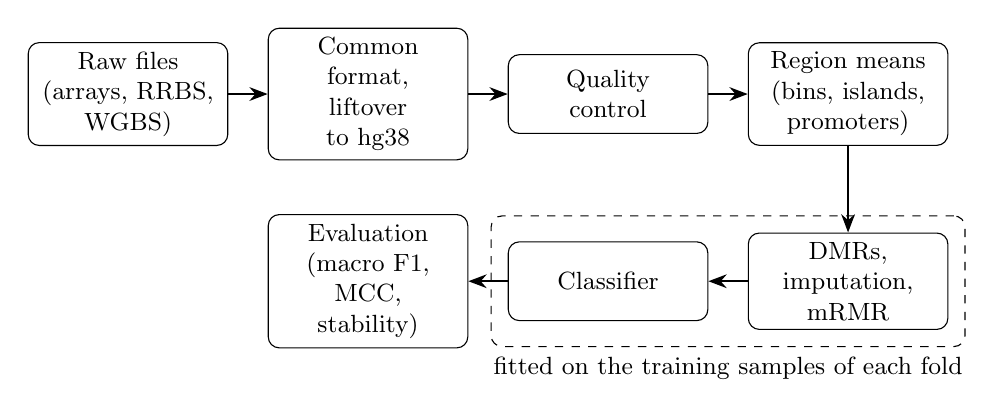
\begin{tikzpicture}[
  box/.style={draw, rounded corners, align=center, font=\small, minimum height=1cm, text width=2.3cm},
  arr/.style={-{Stealth}, thick},
  node distance=0.5cm]
\node[box] (raw) {Raw files\\(arrays, RRBS,\\WGBS)};
\node[box, right=of raw] (fmt) {Common format,\\liftover\\to hg38};
\node[box, right=of fmt] (qc) {Quality\\control};
\node[box, right=of qc] (reg) {Region means\\(bins, islands,\\promoters)};
\node[box, below=1.1cm of reg] (dmr) {DMRs,\\imputation,\\mRMR};
\node[box, left=of dmr] (clf) {Classifier};
\node[box, left=of clf] (eval) {Evaluation\\(macro F1, MCC,\\stability)};
\draw[arr] (raw) -- (fmt);
\draw[arr] (fmt) -- (qc);
\draw[arr] (qc) -- (reg);
\draw[arr] (reg) -- (dmr);
\draw[arr] (dmr) -- (clf);
\draw[arr] (clf) -- (eval);
\node[draw, dashed, rounded corners, fit=(dmr)(clf), inner sep=6pt, label={[font=\small]below:fitted on the training samples of each fold}] {};
\end{tikzpicture}
\caption{Overview of the pipeline.}
\label{fig:pipeline}
\end{figure}

\subsection{Data Used}
Three sets of data are relevant. The \emph{baseline dataset} contains 315 samples from eight classes of the WHO classification~\cite{alaggio2022} (DLBCL, follicular lymphoma, follicular-DLBCL, marginal zone lymphoma, CLL/SLL, T-cell lymphoma, mantle cell lymphoma and normal plasma cell-free DNA), measured with methylation arrays (450K, EPIC), RRBS, WGBS and EM-seq; it is not public and motivates the design of the pipeline. The \emph{validation data} are larger public datasets and, if available, a subset of the baseline data (Section~\ref{sec:validation}). The \emph{case-study dataset} contains 27 public samples from GEO with three classes and three platforms (Section~\ref{sec:case}); it is used to illustrate the methodology.

\subsection{What the Results Are Compared With}
The results are compared (i)~with the baseline pipeline, which identifies DMRs on the whole dataset and evaluates XGBoost on a single 252/63 split; (ii)~between the feature extraction strategies of this work, under the same protocol; (iii)~between the leakage-free and the leaky evaluation of the same pipeline; and (iv)~with the methods reported in the literature (Section~\ref{sec:related}).

\subsection{Data Model and Notation}
A dataset is a set of samples $S=\{s_1,\dots,s_n\}$ with a class $y(s)\in\mathcal{Y}$, a platform $p(s)$, a source dataset $d(s)$ and a sample type $t(s)\in\{\text{tissue},\text{plasma}\}$. After conversion, a sample is a set of measurements
\[
s=\{(c_j, b_j, \sigma_j, n_j, m_j)\}_{j},
\]
where $c_j$ is the chromosome, $b_j\geq 1$ the 1-based position of the cytosine on the genome build hg38, $\sigma_j\in\{+,-,*\}$ the strand, $n_j$ the coverage (number of reads; undefined for arrays) and $m_j\in[0,100]$ the methylation percentage. The strand is $*$ when it is unknown or when the two strands of a CpG were combined.

\subsection{Conversion to the Common Format}
Every input format is converted by its own reader:
\begin{itemize}
\item \textbf{Arrays.} $m_j=100\,\beta_j$ if the values are in $[0,1]$ ($\beta$ values), otherwise $m_j=\beta_j$; $\sigma_j=*$ and $n_j$ is undefined.
\item \textbf{WGBS (BED).} A line $(c,a,e,k,n)$ with the 0-based start $a$, $k$ methylated reads and $n$ reads gives $b=a+1$ and $m=100\,k/n$.
\item \textbf{RRBS (methylKit format~\cite{akalin2012}, with or without header).} A measurement on the reverse strand is reported at the G of the CpG, one base after the C. With strand merging, the two measurements of a CpG are combined with weights given by their coverage:
\[
b = b^{+},\qquad n = n^{+}+n^{-},\qquad m = \frac{n^{+}m^{+}+n^{-}m^{-}}{n^{+}+n^{-}}.
\]
\end{itemize}
Samples on hg19 are moved to hg38 with the UCSC chain file~\cite{kent2002}: a chain is a list of aligned blocks $[a_k,e_k)$ with offsets $o_k$, and a position inside a block is mapped to $b+o_k$. Positions outside every block, in blocks mapped to another chromosome or strand, or mapped onto the same target CpG as another position are removed.

\subsection{Quality Control}
Optionally, only the CpGs of a target panel such as the Twist Human Methylome Panel~\cite{twist2025} are kept. Measurements with coverage below $n_{\min}$ are removed; the threshold can differ by dataset, because plasma cell-free DNA is sequenced with a much lower depth than tumour tissue. A sample is flagged as suspicious when, compared with the other samples of the \emph{same platform}, its median coverage is below a quarter of the platform median or one of its statistics (mean methylation, fraction of CpGs at 0\% and at 100\%) lies more than 3.5 robust deviations from the platform median:
\[
z(x_s)=\frac{x_s-\operatorname{med}(x)}{1.4826\cdot\operatorname{med}\bigl(|x-\operatorname{med}(x)|\bigr)}.
\]
The median and the median absolute deviation are used because, with few samples, a single bad sample inflates the standard deviation and hides itself.

\subsection{Region Features}
A region $r=(c,a,e)$ is a closed interval on a chromosome. Three kinds of regions are used: bins of 1000 bp covering the genome, CpG islands and promoters (from 1500 bp upstream to 500 bp downstream of each transcription start site, on the strand of the gene), the last two from the UCSC tables~\cite{kent2002}. The value of a region in a sample is the mean methylation of the CpGs measured in it,
\[
v_r(s)=\frac{1}{|C_r(s)|}\sum_{j\in C_r(s)} m_j,\qquad C_r(s)=\{j: c_j=c,\ a\leq b_j\leq e\},
\]
and is defined only if $|C_r(s)|\geq \kappa_{p(s)}$. The minimum number of CpGs $\kappa_p$ depends on the platform: arrays measure far fewer CpGs than sequencing, so a threshold suited to sequencing would remove almost all regions of array samples. The values $v_r(s)$ do not depend on the classes or on the folds, so they are computed once per sample and cached.

\subsection{Identification of Differentially Methylated Regions}
For a set of training samples $T$ and a class $k$, the mean of region $r$ is the average of the sample means, so that every sample has the same weight:
\[
\mu_{r,k}=\frac{1}{|T_{r,k}|}\sum_{s\in T_{r,k}} v_r(s),\qquad T_{r,k}=\{s\in T: y(s)=k,\ v_r(s)\text{ defined}\},
\]
kept only if $|T_{r,k}|\geq \phi\,|\{s\in T: y(s)=k\}|$ (by default $\phi=0.5$). A region is a DMR if two classes differ by at least $\delta$ percentage points:
\[
\mathrm{DMR}(T)=\{r: \exists\, k\neq l,\ |\mu_{r,k}-\mu_{r,l}|\geq\delta\}.
\]
All pairs of classes are compared, so the definition works for any number of classes. The alternative strategy \emph{all regions} keeps every region measured in at least a fraction $\phi$ of the training samples and leaves the choice of the informative ones to the feature selection.

\subsection{Feature Selection}
The feature matrix $X\in\mathbb{R}^{|T|\times|\mathrm{DMR}(T)|}$ contains the values $v_r(s)$. Fitted on $T$ only, the selection (i)~removes the features missing in more than 20\% of the samples, (ii)~imputes the remaining missing values with the training median, (iii)~removes the 20\% of the features with the lowest variance and (iv)~chooses $K$ features with mRMR~\cite{ding2005}. The features are discretized into five equal-frequency bins; the first feature maximizes the mutual information $I(f;y)$ with the class, and every next feature maximizes the MIQ criterion
\[
f^{*}=\arg\max_{f\notin F}\ \frac{I(f;y)}{\frac{1}{|F|}\sum_{g\in F} I(f;g)},
\]
where $F$ is the set of features already chosen.

\subsection{Classification}
The selected features are classified with XGBoost~\cite{chen2016} (200 trees, depth 10), random forest~\cite{breiman2001}, an RBF support vector machine~\cite{cortes1995} or L1-regularized logistic regression. Because the classes are strongly imbalanced~\cite{he2009}, all of them use balanced class weights, $w_k=\frac{|T|}{|\mathcal{Y}|\,|T_k|}$, so that the small classes are not ignored.

\subsection{Evaluation Protocol}
Cross-validation~\cite{kohavi1995} becomes optimistic when feature or model selection is done outside the validation loop~\cite{varma2006,cawley2010}; Algorithm~\ref{alg:ncv} therefore shows a nested cross-validation. Every data-dependent step (DMRs, imputation, variance filter, mRMR) is fitted on the training samples of the fold, and the number of features $K$ is chosen in the inner loop. The folds are stratified; if the smallest class has fewer samples than folds, the number of folds is reduced to its size. In the \emph{leaky} variant, used only for comparison, the DMRs and the selected features are computed on all samples before the split.

\begin{algorithm}[!htb]
\caption{Leakage-free nested cross-validation.}
\label{alg:ncv}
\begin{algorithmic}[1]
\Require samples $S$, classes $y$, grid $G$ of values of $K$, $k_{out}$ and $k_{in}$ folds
\For{each outer fold $(T,V)$ of $S$, stratified by $y$}
  \For{each inner fold $(T',V')$ of $T$}
    \State $R'\gets\mathrm{DMR}(T')$; build $X_{T'}$, $X_{V'}$ on $R'$
    \For{each $K\in G$}
      \State fit selection and classifier on $X_{T'}$; record macro F1 on $X_{V'}$
    \EndFor
  \EndFor
  \State $K^{*}\gets$ value of $K$ with the highest mean inner macro F1
  \State $R\gets\mathrm{DMR}(T)$; fit selection with $K^{*}$ and classifier on $X_T$
  \State predict $V$; store the predictions and the selected features $F_V$
\EndFor
\State \Return metrics over folds (mean, standard deviation) and stability of $\{F_V\}$
\end{algorithmic}
\end{algorithm}

\paragraph{Metrics.} With $\mathrm{F1}_k$ the F1 score of class $k$, the macro F1 is $\frac{1}{|\mathcal{Y}|}\sum_k\mathrm{F1}_k$. The multi-class Matthews correlation coefficient~\cite{chicco2020} is computed from the confusion matrix $C$:
\[
\mathrm{MCC}=\frac{c\,s-\sum_k p_k t_k}{\sqrt{\bigl(s^2-\sum_k p_k^2\bigr)\bigl(s^2-\sum_k t_k^2\bigr)}},
\]
where $c$ is the number of correct predictions, $s$ the number of samples, and $t_k$ and $p_k$ the numbers of samples of true and predicted class $k$. The stability of the selected features is the mean pairwise Jaccard index $\frac{2}{q(q-1)}\sum_{i<j}\frac{|F_i\cap F_j|}{|F_i\cup F_j|}$ over the $q$ folds~\cite{nogueira2018}. The grouping of the samples is measured, on the first principal components of the standardized region values, with the silhouette~\cite{rousseeuw1987} of each known grouping and with the adjusted Rand index (ARI)~\cite{hubert1985} between the grouping and a Ward clustering~\cite{ward1963}.

\subsection{Experiments}
Table~\ref{tab:experiments} defines the experiments that test the hypotheses of Section~\ref{sec:hypotheses}; E1 and E2 check the data, E3--E5 test H1--H3, and E0 and E6 need larger data.

\begin{table}[!htb]
\centering
\caption{Experiments.}
\label{tab:experiments}
\small
\begin{tabular}{l>{\raggedright\arraybackslash}p{3.4cm}>{\raggedright\arraybackslash}p{4.2cm}>{\raggedright\arraybackslash}p{4.8cm}}
\toprule
Exp. & Goal & Compared with & Measured \\
\midrule
E0 & Reproduction of the baseline & Results of the baseline pipeline & Macro F1, MCC on the 252/63 split \\
E1 & Correctness of the conversion & Original values (unit tests); other samples of the platform & Per-sample statistics; flagged samples \\
E2 & Overlap of platforms & -- & Regions measured by each platform and shared \\
E3 & Natural grouping (H1) & Grouping by platform and sample type & Silhouette and ARI for class vs.\ platform; UMAP \\
E4 & Feature extraction strategies (H2) & DMRs on bins & Macro F1, MCC, standard deviation over folds, Jaccard stability \\
E5 & Evaluation protocol (H3) & Leaky protocol & Difference in macro F1 and MCC \\
E6 & Generalization across datasets & Standard cross-validation & Macro F1 on the held-out dataset, for classes present in several datasets \\
\bottomrule
\end{tabular}
\end{table}

\subsection{Implementation and Architecture}
The pipeline is implemented in Python as a package. Pandas and NumPy handle the data, scikit-learn~\cite{pedregosa2011} and XGBoost the models, UMAP~\cite{mcinnes2018} the embeddings and Matplotlib the figures. Figure~\ref{fig:architecture} shows the architecture. The steps that have several interchangeable variants are interfaces with one class per variant, registered under a name: a new input format, a new region type or a new region selection method needs a new class and an entry in a configuration file, without changes to the rest of the code. The steps with a single variant (quality control, metrics) are plain functions. The feature selection and the classifiers follow the scikit-learn interface (\texttt{fit}, \texttt{transform}, \texttt{predict}), so any compatible model can be used inside the nested cross-validation. The datasets and the experiments are described in two YAML files.

\begin{figure}[!htb]
\centering
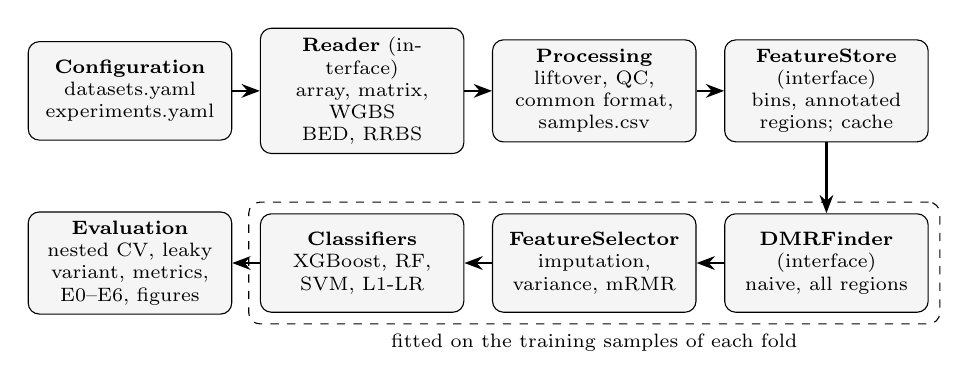
\begin{tikzpicture}[
  mod/.style={draw, rounded corners, align=center, font=\scriptsize, minimum height=1.25cm, text width=2.35cm, fill=gray!8},
  arr/.style={-{Stealth}, thick},
  node distance=0.35cm]
\node[mod] (cfg) {\textbf{Configuration}\\datasets.yaml\\experiments.yaml};
\node[mod, right=of cfg] (read) {\textbf{Reader} (interface)\\array, matrix,\\WGBS BED, RRBS};
\node[mod, right=of read] (proc) {\textbf{Processing}\\liftover, QC,\\common format,\\samples.csv};
\node[mod, right=of proc] (store) {\textbf{FeatureStore}\\(interface)\\bins, annotated\\regions; cache};
\node[mod, below=0.9cm of store] (dmr) {\textbf{DMRFinder}\\(interface)\\naive, all regions};
\node[mod, left=of dmr] (sel) {\textbf{FeatureSelector}\\imputation,\\variance, mRMR};
\node[mod, left=of sel] (clf) {\textbf{Classifiers}\\XGBoost, RF,\\SVM, L1-LR};
\node[mod, left=of clf] (ev) {\textbf{Evaluation}\\nested CV, leaky\\variant, metrics,\\E0--E6, figures};
\draw[arr] (cfg) -- (read);
\draw[arr] (read) -- (proc);
\draw[arr] (proc) -- (store);
\draw[arr] (store) -- (dmr);
\draw[arr] (dmr) -- (sel);
\draw[arr] (sel) -- (clf);
\draw[arr] (clf) -- (ev);
\node[draw, dashed, rounded corners, fit=(dmr)(sel)(clf), inner sep=4pt, label={[font=\scriptsize]below:fitted on the training samples of each fold}] {};
\end{tikzpicture}
\caption{Architecture of the implementation. Boxes marked as interfaces have one class per variant, chosen by name in the configuration.}
\label{fig:architecture}
\end{figure}

The implementation is verified by 101 unit tests (Table~\ref{tab:tests}), run on small synthetic data and on fragments of the real input files. Two tests check properties that the method depends on: that the same CpG gets the same position after conversion from every format, and that the DMRs of a fold are computed only from its training samples.

\begin{table}[!htb]
\centering
\caption{Unit tests of the implementation.}
\label{tab:tests}
\small
\begin{tabular}{>{\raggedright\arraybackslash}p{3.6cm}r>{\raggedright\arraybackslash}p{9cm}}
\toprule
Part & Tests & Examples of what is checked \\
\midrule
Conversion and processing & 40 & 1-based positions, merged strands, scales, liftover, configuration errors, no re-reading of processed samples \\
Quality control & 6 & panel intervals (0-based BED), coverage threshold \\
Regions and DMRs & 25 & bins, CpG islands and promoters, platform-specific density, equal weight of samples, all pairs of classes \\
Feature selection & 8 & mutual information, mRMR, training-only imputation \\
Classifiers and evaluation & 14 & DMRs only from training samples, fold reduction for small classes, nested CV \\
Experiments & 8 & E0--E5 end to end, flagging of suspicious samples \\
\midrule
Total & 101 & \\
\bottomrule
\end{tabular}
\end{table}

The alternatives considered were R and Bioconductor (methylKit~\cite{akalin2012}, DSS~\cite{feng2014}), which offer statistical DMR methods but would split the pipeline between two languages; the Python packages pyranges and pyliftover, replaced by vectorized interval searches that need no extra dependency and are faster on millions of CpGs; and pymrmr, replaced by an own implementation of mRMR that installs on every operating system and can be tested. DSS and the autoencoder~\cite{hinton2006} of the baseline can be added later as another region selection class and another feature selection step.

\section{Case Study}\label{sec:case}

\subsection{Data}
Because the baseline dataset is not public, the case study uses public data from GEO that reproduce the composition of the first, small dataset of the baseline (Table~\ref{tab:case}). Only the samples at diagnosis were kept from GSE66329, since the relapse samples come from the same patients and would let the model recognize the patient instead of the disease; only the tissue samples before treatment were kept from GSE214980, since azacitidine changes DNA methylation; and only the healthy controls were kept from GSE164600.

\begin{table}[!htb]
\centering
\caption{Data of the case study.}
\label{tab:case}
\small
\begin{tabular}{llllllr}
\toprule
Class & GEO series & Study & Platform & Build & Type & Samples \\
\midrule
DLBCL & GSE66329 & Pan et al.~\cite{pan2015} & ERRBS & hg19 & tissue & 11 \\
T-cell lymphoma & GSE214980 & Ruan et al.~\cite{ruan2023} & RRBS & hg19 & tissue & 5 \\
Normal & GSE164600 & Caggiano et al.~\cite{caggiano2021} & WGBS & hg38 & plasma & 11 \\
\midrule
Total & & & & & & 27 \\
\bottomrule
\end{tabular}
\end{table}

The T-cell files were produced with Bismark~\cite{krueger2011} and those of DLBCL with an in-house pipeline, both in the methylKit format. The DLBCL and T-cell files were moved from hg19 to hg38 (at most 0.3\% of the CpGs were lost) and filtered at a coverage of at least 10 reads; the plasma samples, sequenced at a median depth of 11--38 reads, were kept at a coverage of at least 1. The Twist Human Methylome Panel~\cite{twist2025}, used by the baseline, was not applied, since it is not part of the public data. Table~\ref{tab:params} lists all parameters of the pipeline used in the case study.

\begin{table}[!htb]
\centering
\caption{Parameters of the pipeline in the case study.}
\label{tab:params}
\small
\begin{tabular}{>{\raggedright\arraybackslash}p{3.2cm}>{\raggedright\arraybackslash}p{11.4cm}}
\toprule
Step & Parameters \\
\midrule
Quality control & coverage $n_{\min}=10$ (RRBS), $n_{\min}=1$ (plasma WGBS); flagged samples: coverage below $0.25\times$ the platform median or robust $|z|>3.5$ \\
Regions & bins of 1000 bp; promoters from $-1500$ to $+500$ bp around the transcription start site; minimum CpGs $\kappa=10$ (bins), $\kappa=3$ (CpG islands, promoters) \\
DMRs & difference $\delta=25$ percentage points; region present in $\phi=0.5$ of the samples of a class; all pairs of classes \\
Feature selection & features missing in more than 20\% of the samples removed; training-median imputation; 20\% lowest-variance features removed; mRMR (MIQ) on 5 equal-frequency bins; $K\in\{20,50\}$ chosen in the inner loop \\
Classifier & XGBoost, 200 trees, maximum depth 10, learning rate 0.1, balanced class weights \\
Evaluation & 5 outer and 3 inner stratified folds; random seed 42 \\
Grouping (E3) & regions measured in 80\% of the samples; 5000 most variable; 10 principal components; Ward clustering into 3 clusters; UMAP with 15 neighbours \\
\bottomrule
\end{tabular}
\end{table}

\subsection{Experimental Setup}
The experiments ran on a laptop with an AMD Ryzen AI 7 350 processor and 31\,GB of RAM, under Windows 11, with Python 3.14, NumPy 2.5.4, pandas 3.1.1, scikit-learn 1.9.1, XGBoost 3.4.1 and Matplotlib 3.11.2. Converting the 28 downloaded samples took 11 minutes, most of it for the plasma WGBS files (about 27 million CpGs each); computing the region values of all samples for bins, CpG islands and promoters took 17 minutes, once; E1--E5 then took 23 minutes in total. All experiments are run with one command from two configuration files, one for the datasets and one for the experiments, with the fixed seed 42. Every experiment saves, next to its tables and figures, the configuration, the git commit of the code and the versions of the packages, so each number in this section can be traced to the code that produced it.

\subsection{E1: Checks of the Converted Data}
The converters are verified by unit tests on fragments of every format: the same CpG has the same position after conversion from array, WGBS and RRBS files, and the strands of RRBS are merged as defined above. On the real data, the RRBS samples contain 2.6--4.5 million CpGs with a mean methylation of 39--52\%, and the plasma samples 26--27 million CpGs with a mean methylation of 79--81\%. The quality control flagged one of the 12 plasma controls (CTRL11): its median coverage was 2 reads, against 11--38 for the others, and 74\% of its CpGs were at exactly 100\%, against 15--38\%. It was excluded through the configuration file, so the exclusion is documented and can be reverted.

\subsection{E2: Overlap of the Platforms}
Table~\ref{tab:e2} shows the regions measured in at least half of the samples of each platform. The RRBS data cover far fewer regions than WGBS, but almost all of them (96--97\%) are also measured by WGBS. The low Jaccard index of the bins only reflects the much larger number of bins measured by WGBS; the share of RRBS regions also measured by WGBS is the more relevant measure for combining the platforms. CpG islands are the regions shared best by the two platforms (Jaccard index 0.86).

\begin{table}[!htb]
\centering
\caption{E2: regions measured by each platform.}
\label{tab:e2}
\small
\begin{tabular}{lrrrrr}
\toprule
Regions & RRBS & WGBS & Shared & RRBS regions in WGBS & Jaccard \\
\midrule
Bins (1000 bp) & 65\,395 & 973\,503 & 62\,553 & 95.7\% & 0.06 \\
CpG islands & 24\,220 & 26\,145 & 23\,307 & 96.2\% & 0.86 \\
Promoters & 23\,597 & 46\,173 & 22\,954 & 97.3\% & 0.49 \\
\bottomrule
\end{tabular}
\end{table}

\subsection{E3: Natural Grouping of the Samples}
In the UMAP embedding (Fig.~\ref{fig:umap}) the plasma samples are clearly separated from the tumours, and DLBCL and T-cell lymphoma are partly separated. The silhouette is 0.32 for the class and 0.28 for the platform; the ARI of a Ward clustering is 0.22 for the class and 0.07 for the platform. The samples therefore group slightly more by class than by platform, but in this dataset the class coincides with the source dataset, so the two cannot be distinguished.

\begin{figure}[!htb]
\centering
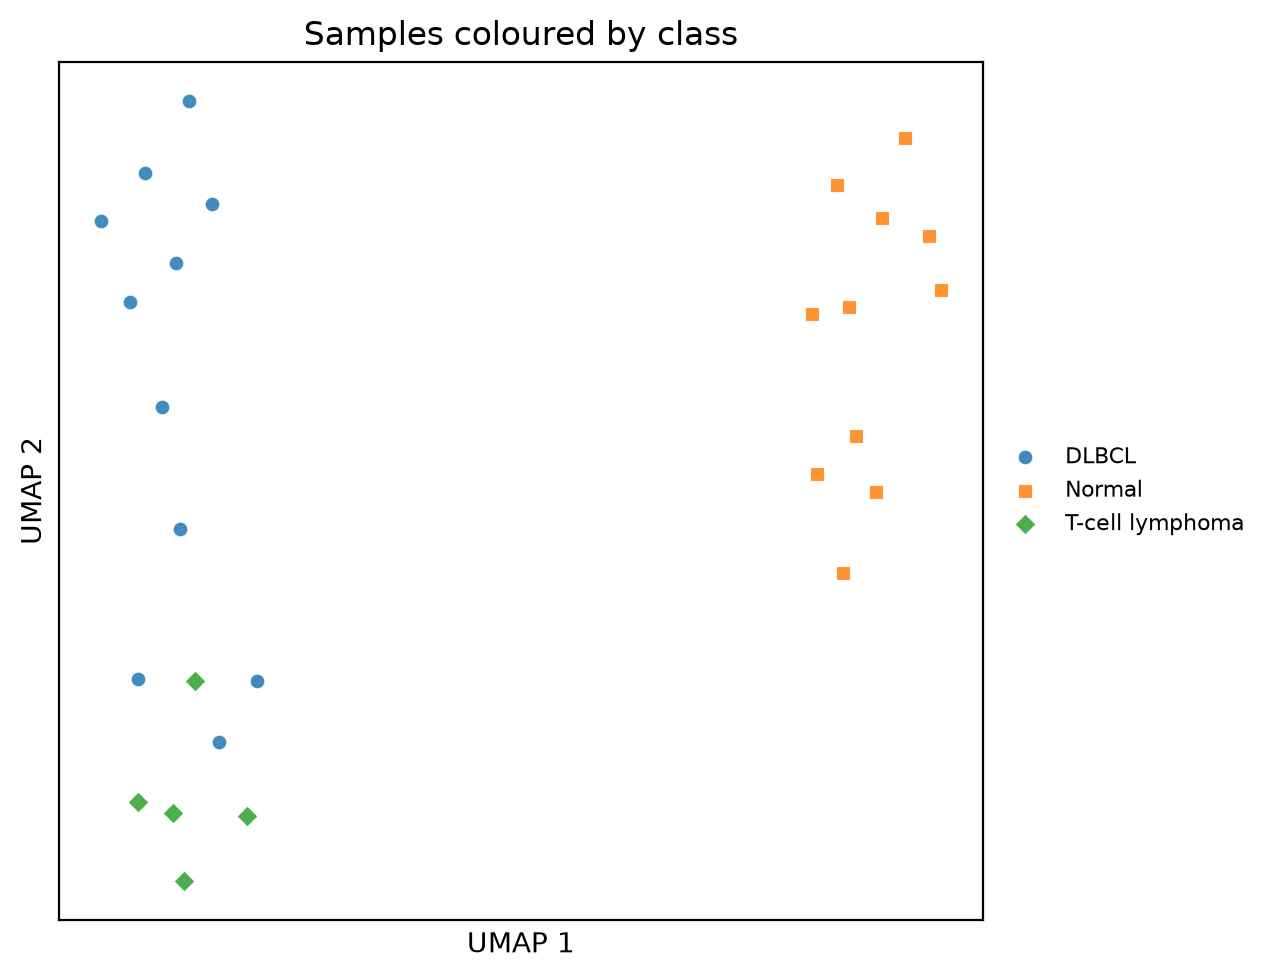
\includegraphics[width=0.48\textwidth]{embedding_class.png}\hfill
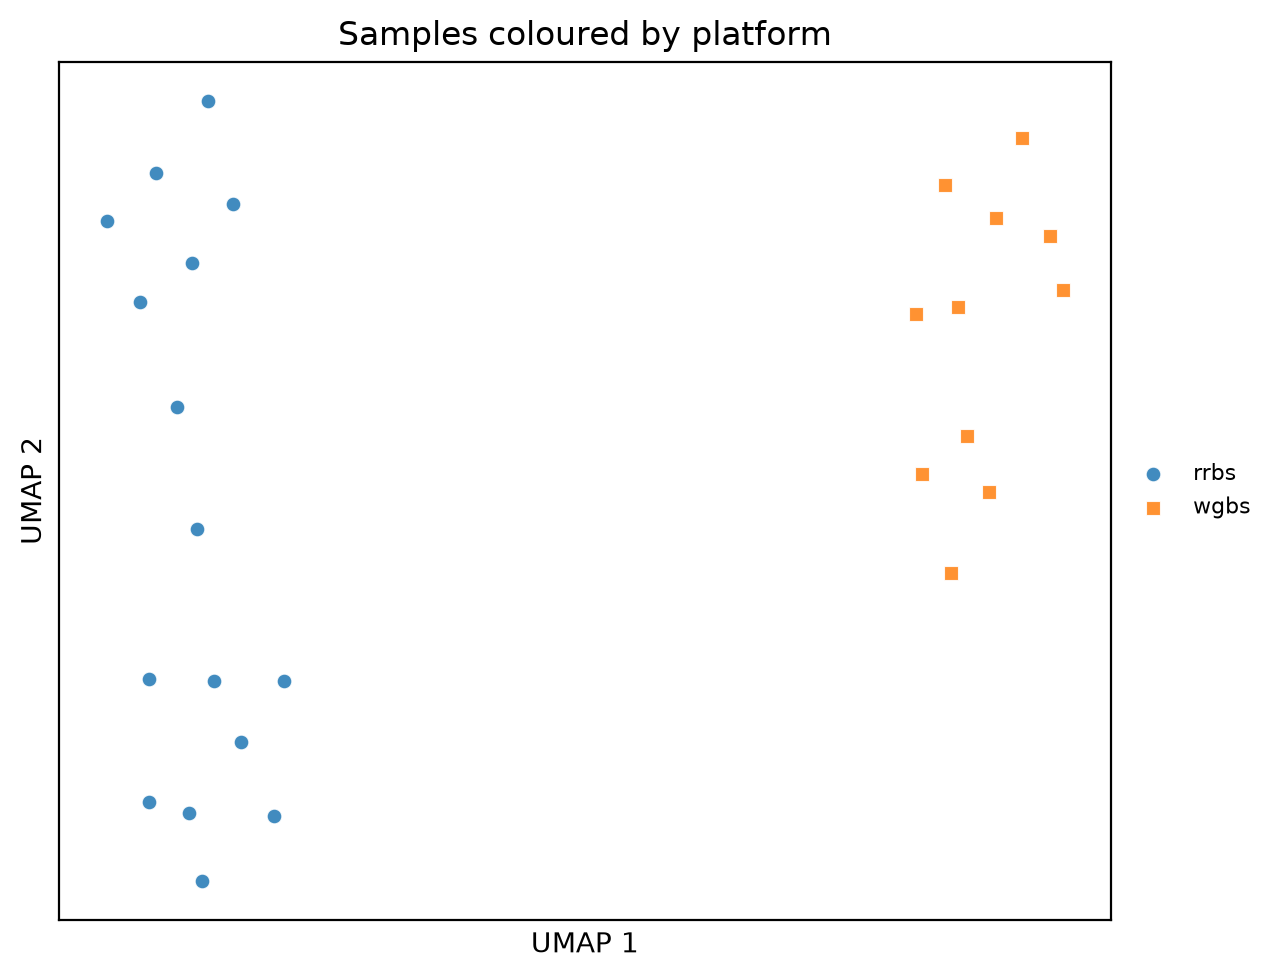
\includegraphics[width=0.48\textwidth]{embedding_platform.png}
\caption{E3: UMAP embedding of the samples, coloured by class (left) and by platform (right).}
\label{fig:umap}
\end{figure}

\subsection{E4: Feature Extraction Strategies}
Table~\ref{tab:e4} compares the strategies under the same nested cross-validation. The best and least variable result is obtained with all CpG islands, without the DMR filter (macro F1 $0.93\pm0.10$). DMRs on bins and on promoters give the same macro F1 ($0.89$), while DMRs on CpG islands are clearly worse ($0.68$), probably because the threshold of 25 points keeps few islands, whose methylation varies less than that of bins. The strategies based on bins, promoters and all CpG islands misclassified two of the 27 samples each, but not the same ones. With DMRs on bins, one plasma control (CTRL10) and one T-cell lymphoma (PTCL4) were predicted as DLBCL; with all CpG islands, all five T-cell samples were recognized, while another plasma control (CTRL2) was predicted as DLBCL and one DLBCL sample (15D1) as T-cell lymphoma. The latter has the lowest median coverage of the DLBCL samples (25 reads, against 59--100), so its region values are the noisiest. The stability of the selected features is low for all strategies (0.05--0.15): with 27 samples and thousands of correlated regions, every fold chooses different but equivalent features. The standard deviations over the five folds (0.10--0.21) are of the same order as the differences between the strategies, so only the lower result of DMRs on CpG islands can be considered a clear difference; the others need repeated cross-validation and a statistical test to be separated.

\begin{table}[!htb]
\centering
\caption{E4: comparison of the feature extraction strategies (mean $\pm$ standard deviation over 5 outer folds).}
\label{tab:e4}
\small
\begin{tabular}{lrrrr}
\toprule
Strategy & Candidate regions & Macro F1 & MCC & Stability \\
\midrule
DMRs on bins & 12\,795 & $0.89\pm0.18$ & $0.90\pm0.14$ & 0.05 \\
DMRs on CpG islands & 4\,209 & $0.68\pm0.21$ & $0.68\pm0.24$ & 0.15 \\
DMRs on promoters & 5\,861 & $0.89\pm0.17$ & $0.90\pm0.14$ & 0.06 \\
All CpG islands & 24\,746 & $0.93\pm0.10$ & $0.90\pm0.13$ & 0.05 \\
\bottomrule
\end{tabular}
\end{table}

Table~\ref{tab:perclass} shows the results per class, computed from the predictions of all folds. T-cell lymphoma, the smallest class, is the most difficult one for DMRs on bins, while all CpG islands recognize it completely at the cost of one DLBCL sample.

\begin{table}[!htb]
\centering
\caption{E4: precision, recall and F1 per class over all folds, for two strategies.}
\label{tab:perclass}
\small
\begin{tabular}{lrrrrrrr}
\toprule
 & & \multicolumn{3}{c}{DMRs on bins} & \multicolumn{3}{c}{All CpG islands} \\
\cmidrule(lr){3-5}\cmidrule(lr){6-8}
Class & Samples & Precision & Recall & F1 & Precision & Recall & F1 \\
\midrule
DLBCL & 11 & 0.85 & 1.00 & 0.92 & 0.91 & 0.91 & 0.91 \\
T-cell lymphoma & 5 & 1.00 & 0.80 & 0.89 & 0.83 & 1.00 & 0.91 \\
Normal & 11 & 1.00 & 0.91 & 0.95 & 1.00 & 0.91 & 0.95 \\
\bottomrule
\end{tabular}
\end{table}

\subsection{E5: Leakage-Free versus Leaky Evaluation}
Table~\ref{tab:e5} shows the same pipeline evaluated with and without information leakage. The difference is negligible ($-0.01$ macro F1, $+0.004$ MCC). In the leaky protocol the selected features are identical in every fold (stability 1), but the predictions barely change: the classes of this dataset differ so strongly, partly for technical reasons, that the leakage has nothing left to inflate.

\begin{table}[!htb]
\centering
\caption{E5: evaluation with and without information leakage (DMRs on bins).}
\label{tab:e5}
\small
\begin{tabular}{lrrr}
\toprule
Protocol & Macro F1 & MCC & Stability \\
\midrule
Leakage-free & $0.89\pm0.18$ & $0.90\pm0.14$ & 0.05 \\
Leaky & $0.88\pm0.18$ & $0.90\pm0.14$ & 1.00 \\
\bottomrule
\end{tabular}
\end{table}

\subsection{E0 and E6}
E0 needs the data and the split of the baseline, and E6 needs classes present in several datasets; neither is possible on the public data of the case study, in which every class comes from one dataset. Both are prepared for the validation on larger data (Section~\ref{sec:validation}).


\subsection{Verdicts on the Hypotheses}
\begin{itemize}
\item \textbf{H1 (not testable on this dataset).} The samples group slightly more by class than by platform (silhouette 0.32 vs.\ 0.28, ARI 0.22 vs.\ 0.07), but the class coincides with the dataset and, for the normal samples, with the platform and the sample type, so the two effects cannot be separated. The difference in mean methylation between plasma WGBS (79\%) and tumour RRBS (46--51\%) is mostly technical: WGBS measures the whole genome, which is mostly methylated, while RRBS measures mainly CpG islands, which are mostly unmethylated.
\item \textbf{H2 (confirmed for the performance, not for the stability).} All CpG islands, without the DMR filter, give the best macro F1 ($0.93\pm0.10$) and are the regions shared best by the platforms. Their selected features are, however, not more stable (Jaccard 0.05). With 25 of 27 samples correct, the accuracy of this strategy is 0.93 with a 95\% Wilson interval of $[0.77, 0.98]$, which overlaps the interval of DMRs on bins (also 25 of 27); only DMRs on CpG islands (21 of 27, interval $[0.59, 0.89]$) are clearly worse.
\item \textbf{H3 (not confirmed on this dataset).} The leaky protocol changed the macro F1 by $-0.01$ and the MCC by $+0.004$. The effect of leakage is expected where the signal is weak, e.g.\ between lymphoma subtypes measured on the same platform, which this dataset does not contain.
\end{itemize}

\subsection{Threats to Validity}
\begin{enumerate}
\item \textbf{Missing baseline.} The pipeline was not compared directly with the baseline (E0), because its data and its train/test split are not public; the comparison with the literature is qualitative (Section~\ref{sec:related}).
\item \textbf{Confounding.} Every class comes from a different laboratory, platform and genome build, so the classifiers may partly separate the datasets instead of the diseases; leave-one-dataset-out evaluation (E6) was not possible.
\item \textbf{Sample size.} With 27 samples, five of them T-cell lymphomas, every outer fold contains one T-cell sample, the standard deviations over folds are 0.10--0.21 and the 95\% intervals of the accuracy are about 0.2 wide; the differences between the three best strategies are within this uncertainty.
\item \textbf{Fixed parameters.} The DMR threshold ($\delta=25$), the density thresholds and the bin size were fixed in advance, as in the baseline, and not tuned; other values may change the ranking of the strategies.
\item \textbf{Data processing.} The liftover from hg19 to hg38 removed at most 0.3\% of the CpGs, the Twist panel was not applied, and one plasma control with very low coverage was excluded after quality control.
\end{enumerate}
The results therefore illustrate the methodology and are not a claim about the biology of the lymphomas. The next step is the validation on larger data described in Section~\ref{sec:validation}, which addresses the first three threats: more samples per class, classes measured in several datasets for E6, and, if the data become available, a direct comparison with the baseline.

\bibliographystyle{splncs04}
\bibliography{references}

\end{document}